\section{Comparing RLS implementations}
To compare between both implementations, I will be using the same dataset for all runs. The forgetting rate will be set to 0.98, and the P initialisation value $\epsilon$ will be set to 0.1.
The setup for this experimentation will the same as in Tasks 1 \& 2 to take advantage of the prior knowledge of true weights for the dataset.
\subsection{Original Padasip Implementation}
Padasip provides values that have a much wider variance than my implementation, these error  values are also much higher than the error values produced by my own implementation.

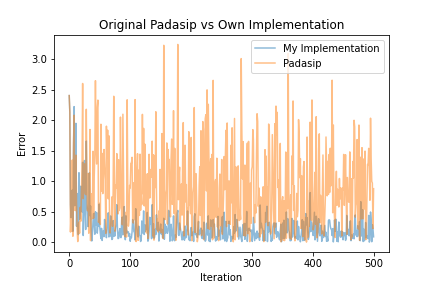
\includegraphics[width=\linewidth]{figs/OrigPadasip.png}

Comparing the found weights MSE compared to their true values, this difference in accuracy is apparent.
\begin{center}
    \begin{tabular}{| c c |}
        \hline
        Algorithm & Weight MSE \\ 
        \hline\hline
        Original Padasip & $4.20 \times 10^{-1}$\\ 
        My implementation & $4.71 \times 10^{-3}$\\
        \hline      
    \end{tabular}
\end{center}

\subsection{Modified Padasip Implementation}
It was noted that the Padasip implementation has a bug in it due to the shaping of data, fixing the bug using the provided code provides the following implementation.

When the bug was corrected, the Padasip implementation provided an almost exact result to my implementation.

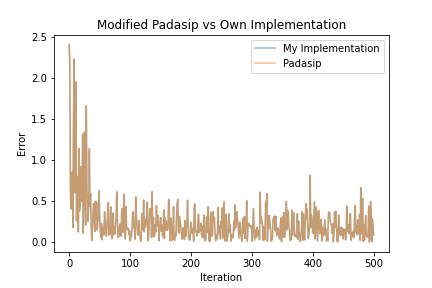
\includegraphics[width=\linewidth]{figs/ModPadasip.png}

The implementations are so close to one another that the MSE between the predictions performed by the two implementations is $2.81 \times 10^{-27}$ compared to 0.91 between my implementation and the original Padasip implementation. 